\subsection{Beispiel}
    \label{section:solutionDetailPersistenceDataModelExample}
    Um das eben beschriebene Datenmodell greifbarer zu machen,
    präsentiert dieses Kapitel, wie eine konkrete Klassifikation als
    Graph im {\classificationStorage} gespeichert wird.
    Spätere Erklärungen nehmen auf dieses Beispiel ebenfalls Bezug.
    Eine Übersicht der Knoten des Beispielgraphs wurde aus Gründen
    der Übersichtlichkeit auf die Abbildungen \ref{image:dbDataModelExampleOverviewPart1}
    und \ref{image:dbDataModelExampleOverviewPart2} verteilt.
    Sie sind über den \texttt{Content}-Knoten \texttt{c5} verbunden
    und verzichten zunächst auf die ausführliche Darstellung der Eigenschaften der Beziehungen.

    \begin{figure}[htb]
        \centering
        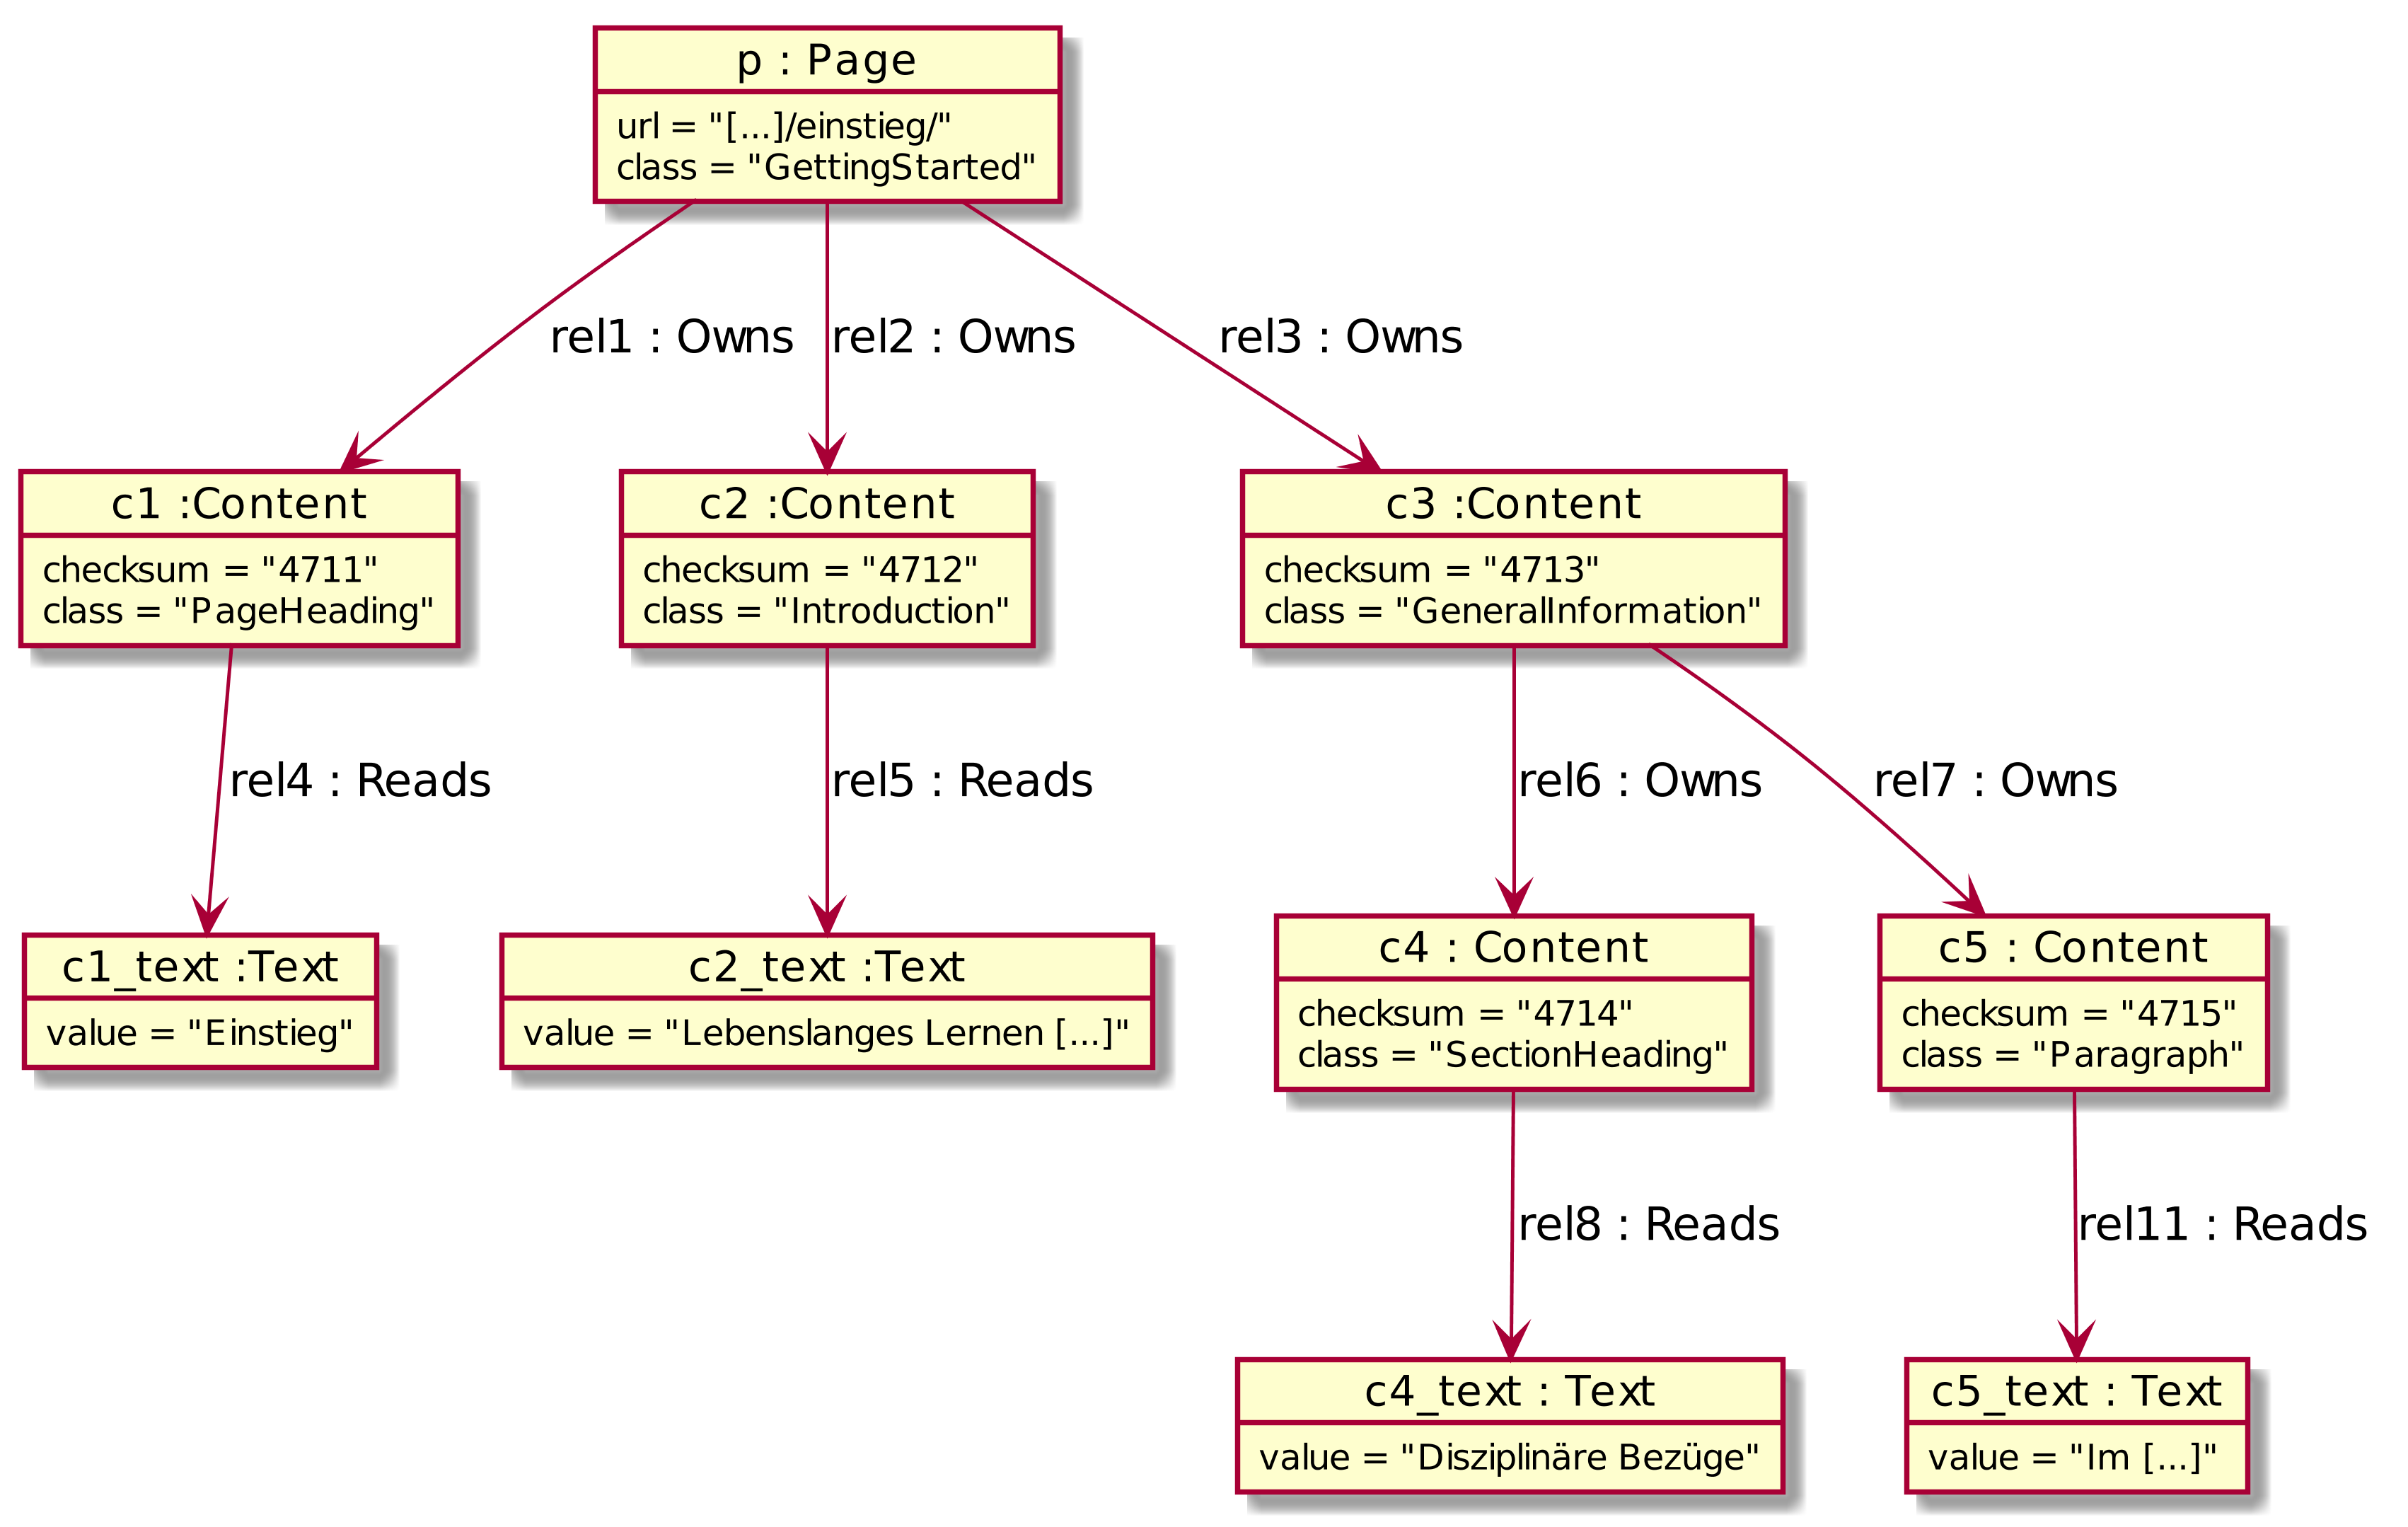
\includegraphics[scale=\imageScalingFactor]{../resources/db-data-model/example/example_part1.png}
        \caption{Beispiel eines Graphs im {\classificationStorage} (1)}
        \label{image:dbDataModelExampleOverviewPart1}
    \end{figure}

    Die betroffene Webseite wurde als "`GettingStarted"' klassifiziert und besitzt drei skalare {\contentFeature}s,
    für die \texttt{Content}-Knoten existieren.
    Der \texttt{Page}-Knoten ist mit ihnen über \texttt{Owns}-Beziehungen verbunden.
    Die Inhalte \texttt{c1} und \texttt{c2} beinhalten Text und sind deshalb mit entsprechenden \texttt{Text}-Knoten verbunden.
    Der Knoten \texttt{c3} hat hingegen zwei {\childFeature}s (\texttt{c4} und \texttt{c5}), die seinen Text feingranular speichern
    und deshalb ihrerseits mit \texttt{Text}-Knoten verbunden sind.
    In Abbildung \ref{image:dbDataModelExampleOverviewPart2} ist zu sehen,
    dass \texttt{c5} neben seinem Text auch zwei {\resources} referenziert,
    die durch entsprechende \texttt{Resource}-Knoten dargestellt werden.

    \begin{figure}[htb]
        \centering
        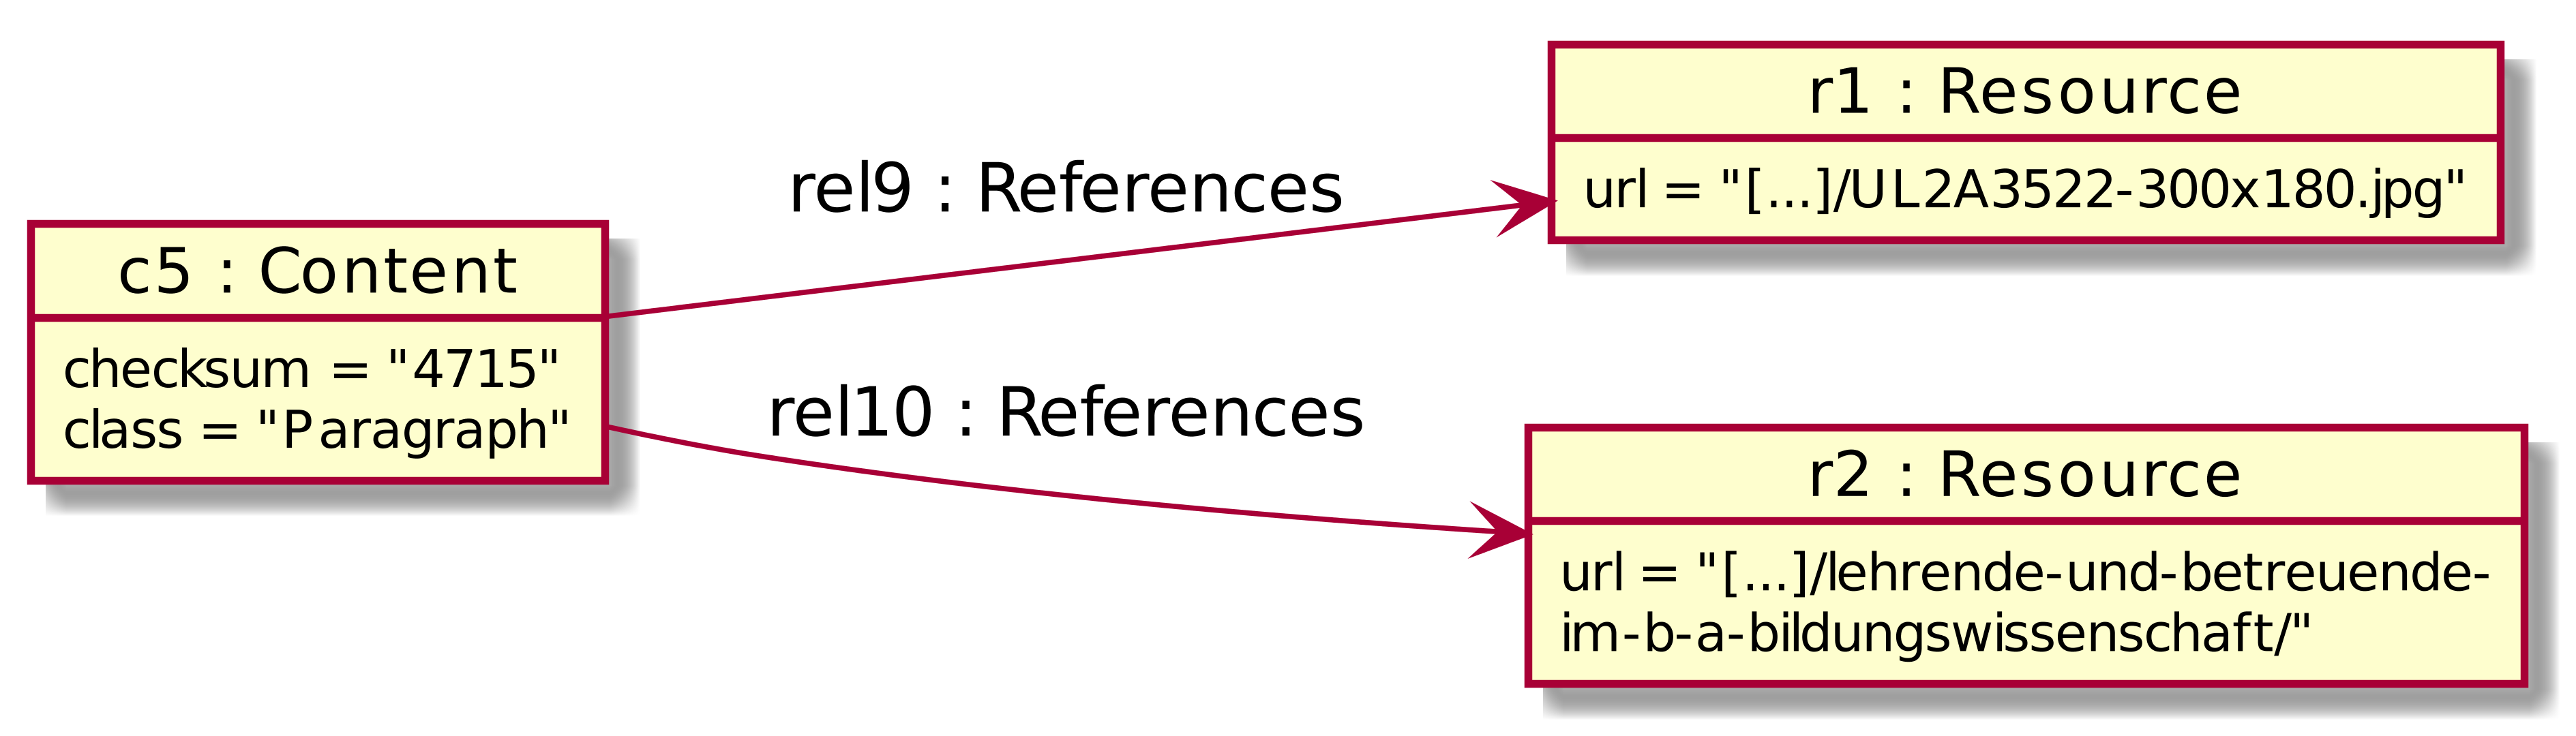
\includegraphics[scale=\imageScalingFactor]{../resources/db-data-model/example/example_part2.png}
        \caption{Beispiel eines Graphs im {\classificationStorage} (2)}
        \label{image:dbDataModelExampleOverviewPart2}
    \end{figure}

    Bei diesen Referenzen handelt es sich um ein {\collectionFeature},
    was aus Abbildung \ref{image:dbDataModelExampleRel10} hervorgeht,
    die eine Beziehung zu einem \texttt{Resource}-Knoten detailliert darstellt.

    \begin{figure}[htb]
        \centering
        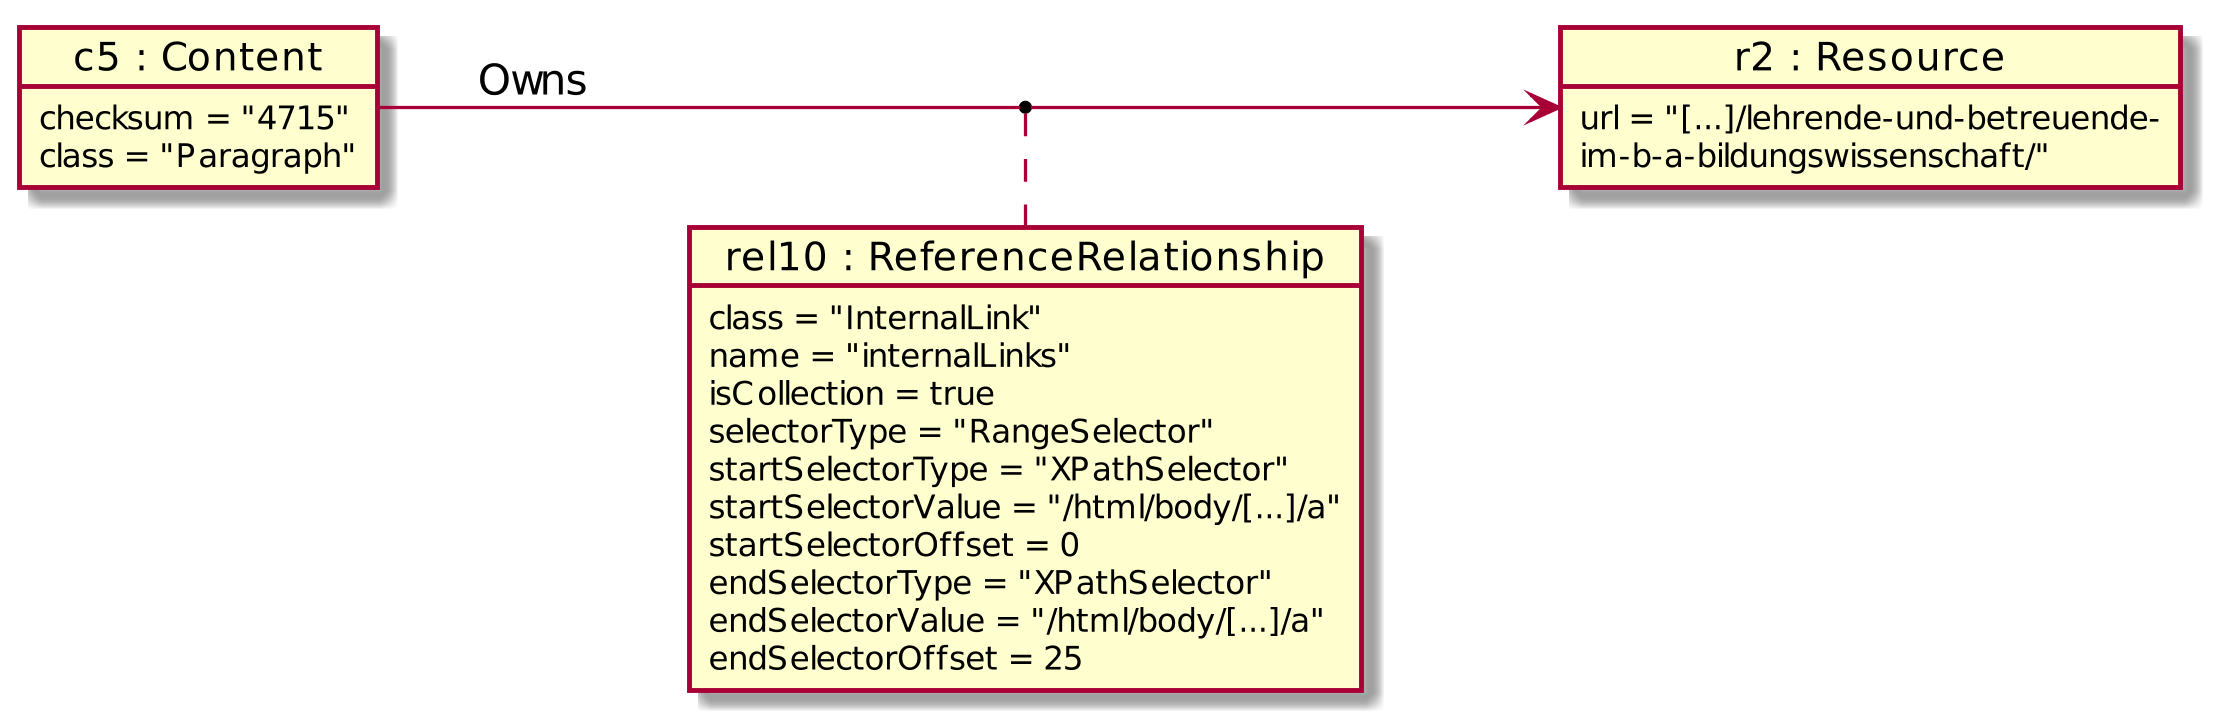
\includegraphics[scale=\imageScalingFactor]{../resources/db-data-model/example/c5-r2.png}
        \caption{Beispiel einer Beziehung zu einer {\resource} im {\classificationStorage}}
        \label{image:dbDataModelExampleRel10}
    \end{figure}

    Die Eigenschaft \texttt{isCollection} besitzt nämlich den Wert \texttt{true}.
    Des Weiteren wird hier deutlich, wie die Informationen des eindeutigen Selektors gespeichert werden.
    Dem Datenmodell folgend ist eine konkrete Beziehung zu einem \texttt{Content}-Knoten
    sehr ähnlich aufgebaut. Wie in Abbildung \ref{image:dbDataModelExampleRel1} zu sehen,
    verzichtet sie lediglich auf die Speicherung der Klasse.

    \begin{figure}[htb]
        \centering
        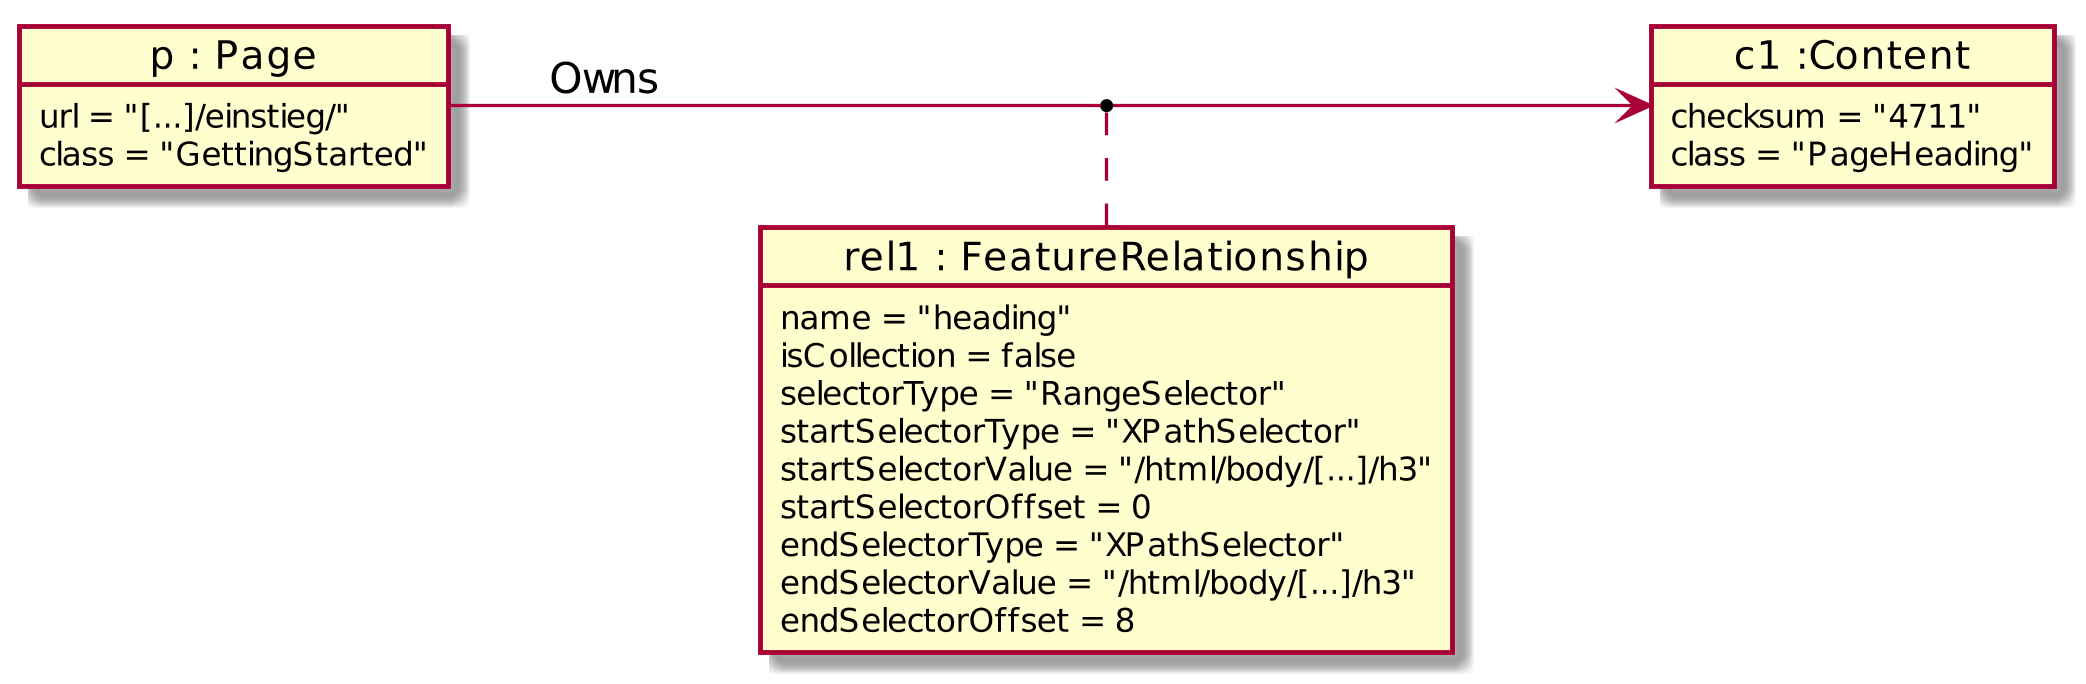
\includegraphics[scale=\imageScalingFactor]{../resources/db-data-model/example/p-c1.png}
        \caption{Beispiel einer Beziehung zu einem {\contentFeature} im {\classificationStorage}}
        \label{image:dbDataModelExampleRel1}
    \end{figure}
